\documentclass{beamer}
\usepackage{caption}
\usepackage[utf8]{inputenc}
\usepackage[english]{babel}
\usepackage{booktabs}
\usepackage{listings}

\lstdefinestyle{C++}{language=C++,
                showstringspaces=false,
                basicstyle=\ttfamily,
                keywordstyle=\color{blue}\ttfamily,
                stringstyle=\color{red}\ttfamily,
                commentstyle=\color{green}\ttfamily,
                morecomment=[l][\color{magenta}]{\#}
}
\lstdefinestyle{shell}{basicstyle=\ttfamily}


\title{(Not yet Adaptive) Compression of In-Memory Databases}
\subtitle{Database Implementation Lab Course}
\author{Leon Windheuser}

\begin{document}

\frame{\titlepage}


\begin{frame}
    \frametitle{Project Introduction}
    Compression of the In-Memory part of DuckDB
    \vspace{1cm}
    \pause

    \begin{itemize}
        \item Open Source SQL OLAP RDBMS 
        \item Columnar Storage format
        \item Vectorized execution engine
        \item Has lots of different compression for persistent data on disk 
    \end{itemize}

    \vspace{1cm}
    \pause
    How do we compress data in-memory while having efficient lookups without decompressing everything?
\end{frame}


\begin{frame}
    \frametitle{Succinct Data Structures}
    
    \begin{itemize}
        \item Data structures which uses close to the \textit{information-theoretic} lower bound of space but 
    allows efficient query operations (in-place without needing to decompress)
        \item Exists for e.g. {\only<+>{bit vectors}\only<+->{\textbf{bit vectors}}}, trees, planar graphs, ...
    \end{itemize}
\end{frame}


\begin{frame}
    \frametitle{Succinct Integer Vector}
    \centering
    Space requirement for integer $x$ is $\ell = \lfloor \log_2(x) \rfloor + 1$ bits

    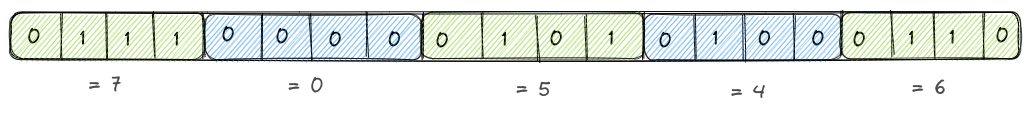
\includegraphics[width=\framewidth]{figures/excalidraw/bit-int-vector.png}
    \pause

    Encode integers with the minimal length of the max integer $3 = \lfloor \log_2(7) \rfloor + 1$ \\
    \vspace{0.5cm} 
    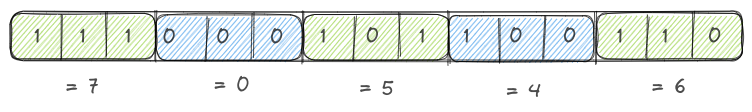
\includegraphics[width=0.75\framewidth]{figures/excalidraw/bit-compressed-int-vector.png}

    \vspace{0.5cm}
    \textbf{We already reduce memory by 25\%}
\end{frame}


\begin{frame}
    \frametitle{SDSL: Succinct Data Structure Library}

    \begin{itemize}
        \item C++11 library and abstraction for succinct data structures
        \item Open Source \url{https://github.com/simongog/sdsl-lite}
        \item Contains varierty of different data structures. For now we only used the \textbf{Integer Vectors}.
    \end{itemize}
\end{frame}


\begin{frame}[fragile]
    \frametitle{SDSL: Integer Vectors}

\begin{lstlisting}[style=C++]
sdsl::int_vector<32> v(10000);
for (size_t i = 0; i < 10000; i++) v[i] = i;
cout << "Width: " << v.width() << ", size: " 
     << sdsl::size_in_bytes(v) << endl;
sdsl::util::bit_compress(v);
cout << "Width: " << v.width() << ", size: " 
     << sdsl::size_in_bytes(v) << endl;
\end{lstlisting}

\pause

\begin{lstlisting}[style=shell]
Width: 32, size: 40008
Width: 14, size: 17513
\end{lstlisting}

\pause

\begin{center}
    Reduces memory by 56.2\% ($\approx$ 22.5 KB)
\end{center}
\end{frame}


\begin{frame}[fragile]
    \frametitle{Extract min element from \ttfamily{sdsl::int\_vector}}

\begin{lstlisting}[style=C++]
sdsl::int_vector<32> v(10000);
for (size_t i = 0; i < 10000; i++) 
    v[i] = i + 10.000.000;
cout << "Width: " << v.width() << ", size: " 
     << sdsl::size_in_bytes(v) << endl;
sdsl::util::bit_compress(v);
cout << "Width: " << v.width() << ", size: " 
     << sdsl::size_in_bytes(v) << endl;
\end{lstlisting}

\begin{lstlisting}[style=shell]
Width: 32, size: 40008
Width: 24, size: 30008
\end{lstlisting}
\end{frame}


\begin{frame}[fragile]
    \frametitle{Extract min element from \ttfamily{sdsl::int\_vector}}
\begin{lstlisting}[style=C++]
sdsl::int_vector<32> v(10000);
for (size_t i = 0; i < 10000; i++) 
    v[i] = i + 10.000.000;
cout << "Width: " << v.width() << ", size: " 
     << sdsl::size_in_bytes(v) << endl;
extractMinFromVector(v);
sdsl::util::bit_compress(v);
cout << "Width: " << v.width() << ", size: " 
     << sdsl::size_in_bytes(v) << endl;
\end{lstlisting}

\begin{lstlisting}[style=shell]
Width: 32, size: 40008
Width: 14, size: 17513
\end{lstlisting}

\pause
We will know the minimum of the vector / column in databases without searching 
(column statistics)
\end{frame}


\begin{frame}[fragile]
    \frametitle{Random Access of \ttfamily{sdsl::int\_vector[i]} vs \ttfamily{std::vector[i]}}

\end{frame}

\begin{frame}
    \frametitle{Byte-Align \ttfamily{sdsl::int\_vector}}
\end{frame}


\begin{frame}
    \frametitle{DuckDB Storage Architecture 100 meter view}
    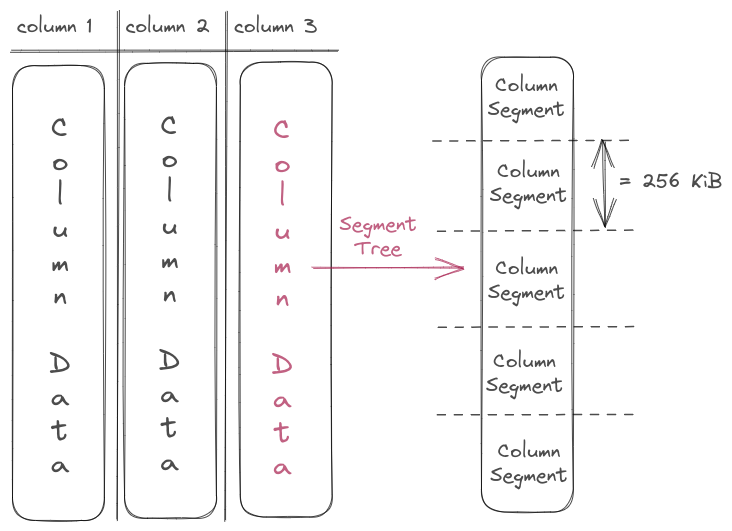
\includegraphics[width=\framewidth]{figures/excalidraw/duckdb-high-level-storage-arch.png}
\end{frame}

\begin{frame}
    \frametitle{DuckDB Storage Architecture 10 meter view}
    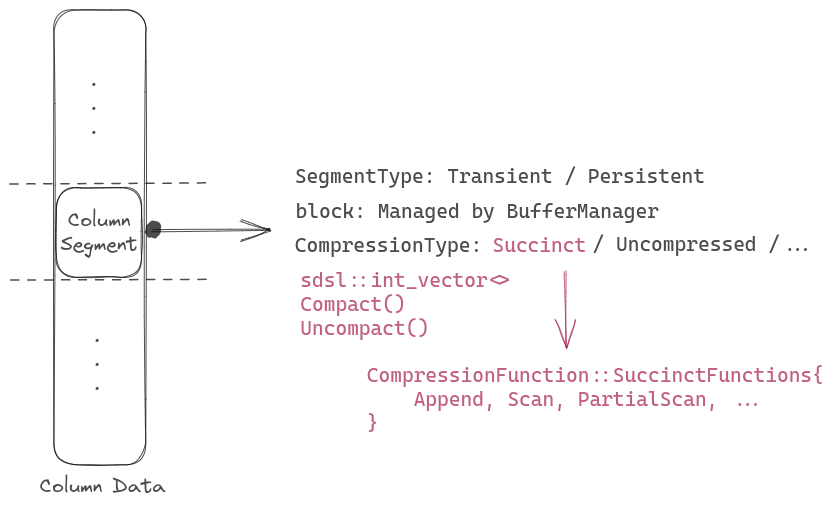
\includegraphics[width=\framewidth]{figures/excalidraw/duckdb-column-segment-look.png}

\end{frame}


\begin{frame}
    \frametitle{Benchmarks}
\end{frame}

\end{document}
